%==============================================================================
% AAMAS 2027 submission -- SUPPLEMENTARY MATERIAL
%
% Deliberately a SECOND DOCUMENT INSIDE THE SAME PROJECT, not a separate
% project and not an appendix to main.tex:
%   * it shares aamas.cls, refs.bib and tables/ with the main paper, so a
%     regenerated table lands in both at once and the two can never disagree;
%   * it stays out of main.tex's page budget, which is measured by
%     scripts/pagecheck.py on main.pdf alone.
%
% Build:  pdflatex supplement && bibtex supplement && pdflatex supplement x2
%
% ANONYMOUS. Same rule as the main paper: no author, institution, repository
% or URL. Run the anonymity gate on THIS pdf too, not only main.pdf.
%
% THE MAIN PAPER MUST REMAIN READABLE WITHOUT THIS FILE. Everything here is
% backing for a claim the main text already states; nothing here is load-
% bearing for the argument. If you find yourself moving an argument step into
% this document, move it back.
%==============================================================================
% balance=false: the class balances the columns of the last page, and doing so
% printed the last two single-column tables out of numerical order.
\documentclass[sigconf,anonymous,balance=false]{aamas}

% -- AAMAS-2027 copyright block, verbatim from AAMAS_2027_sample.tex.
\makeatletter
\gdef\@copyrightpermission{
  \begin{minipage}{0.2\columnwidth}
   \href{https://creativecommons.org/licenses/by/4.0/}{
\includegraphics[width=0.90\textwidth]{by}}
  \end{minipage}\hfill
  \begin{minipage}{0.8\columnwidth}
   \href{https://creativecommons.org/licenses/by/4.0/}{This work is licensed under a Creative Commons Attribution International 4.0 License.}
  \end{minipage}
  \vspace{5pt}
}
\makeatother

\setcopyright{ifaamas}
\acmConference[AAMAS 2027]{Proc.\@ of the 26th International Conference
on Autonomous Agents and Multiagent Systems (AAMAS 2027)}{3--7 May 2027}{Hanoi, Vietnam}{M.~Baldoni, F.~Fang, W.~Yeoh, N.~Yorke-Smith (eds.)}
\copyrightyear{2027}
\acmYear{2027}
\acmDOI{}
\acmISBN{}

% Same OpenReview submission number as main.tex.
\acmSubmissionID{2850}
\submissionType{Research Paper Track}

\usepackage{booktabs}
\usepackage{amsmath}
\usepackage{xcolor}
\microtypesetup{protrusion=false}
\usepackage{etoolbox}


% House style for every table in this document: one font size and one column
% gap, set once here rather than in each generated file; a short caption
% (the class prints captions in bold) and the column definitions in a note
% below the table, set with \tabnote.
\AtBeginEnvironment{table}{\small\setlength{\tabcolsep}{4pt}}
\AtBeginEnvironment{table*}{\small\setlength{\tabcolsep}{4pt}}
\newcommand{\tabnote}[1]{\par\vspace{3pt}\begin{minipage}{\linewidth}\footnotesize\setlength{\parindent}{0pt}#1\par\end{minipage}}

\newcommand{\Pone}{\textsf{P1a}}
\newcommand{\PER}{\textsc{PER}}
% The ACM reference line would run the two-line title together; the
% supplement does not need one.
\settopmatter{printacmref=false}

% Float placement for this document only (the main paper keeps the class
% defaults). Most tables here are page-wide; with the defaults LaTeX holds
% them back and starts float-only pages that are mostly empty. These values
% let a wide table share its page with text and fill float pages further.
\renewcommand{\topfraction}{0.9}
\renewcommand{\dbltopfraction}{0.9}
\renewcommand{\textfraction}{0.07}
\renewcommand{\floatpagefraction}{0.8}
\renewcommand{\dblfloatpagefraction}{0.8}
\setcounter{topnumber}{3}
\setcounter{dbltopnumber}{3}
\setcounter{totalnumber}{4}

\begin{document}

\title{Supplementary Material\\
\large From Feedback to Revision: When Do Multi-Agent Roles Look
Load-Bearing?}

\author{Anonymous Author(s)}
\affiliation{%
  \institution{Anonymous Institution}
  \country{}
}

\maketitle

\section*{What this document is}

The main paper states every claim it makes and is complete without this
file. What it cannot carry in eight pages is the full numeric backing behind
some of its sentences, and that backing is here, in the order of the main
paper's results: the realized organization (R1), recovery (R2), the
submission gate (R3), the second domain (R4) and structural enforcement
(R5), followed by the pre-registered endpoints and the single-agent
comparator. Every table is generated by a script from the manifested data
(the frozen snapshot, or the separately manifested post-freeze runs) with
the same scripts and outputs as the main paper's tables, except the
single-agent comparator, which comes from an earlier, separately collected
corpus. The four figures are generated from the same outputs.

\paragraph{Terms used throughout.} A \emph{trajectory} is one problem's run
through the pipeline, at most six \emph{cycles} of Planner, Executor and
Reviewer. A cycle ends in a \emph{submission} to the evaluator when the
third agent approves the current answer, and in a \emph{decline} otherwise;
each submission returns a \emph{verdict}, PASS or FAIL, and on a FAIL a
repair hint. \emph{First pass} is whether the first submitted answer is
correct; a trajectory that never submits is graded once when its budget
runs out, and that grade is its first pass. \emph{Recovery} is the share of
\emph{first-pass-wrong} trajectories that finish correct. Recovery is
reported on two populations that must not be read across: the
\emph{marginal} population is every first-pass-wrong trajectory of a
condition, on that condition's own denominator; the \emph{paired}
population is only the problems first-pass wrong under both conditions
being compared, on one shared denominator, and it is the population every
test of recovery uses. Tests are exact McNemar tests on the problems that
exactly one condition gets right; intervals are $95\%$ bootstrap intervals
that resample problems; where several tests form a family, $p$ values are
corrected with Holm's step-down procedure. Two \emph{scorings} recur: the
\emph{pre-registered} scoring counts a trajectory that never produced a
graded answer as incorrect, and the \emph{as-graded} scoring drops it. The
conditions are abbreviated RS (role-structured: Planner, Executor and
Reviewer prompts), RF (role-free: one generic prompt for all three agents,
with the evaluator's feedback shown), RF$^{-}$ (role-free with the feedback
withheld) and SE (structurally enforced: the same roles imposed by typed
message formats). The actors are the gemma-4-31B-it, gpt-oss-120b and
Llama-3.3-70B-Instruct models, each playing all three agents.

\section{The realized organization (R1)}
\label{sec:collapse_full}

The main paper reports that deleting the role clauses makes every agent
assert its own final answer. Table~\ref{tab:collapse_full} is the full form
of its Table~1, with two further measures and the enforced condition, and
Figure~\ref{fig:roles} shows which agent changes.

% ==========================================================================
% Supplement -- functional collapse per actor, all three measures
%
% GENERATED FILE -- do not edit by hand. Any edit is overwritten.
% generating script : analysis/scripts/mk_tables.py
% canonical input   : analysis/out/FINAL_TABLES_OUTPUT.txt  sections T1, T18, T20, T23
%                    analysis/out/FIGDATA_BF.json  (role-free with feedback: collapse only)
% frozen data       : experiments/results/FROZEN/, frozen_at 2026-09-30T10:09:30.201557
%                     11600 trajectories
%                     sha256 fa22a446d5314bb67b1c6a6444b511eeeae3eb8770419a36f182617eeccbf3b5  actor3.jsonl
%                     sha256 038e08aec4d4aee166106a6325309dfe2301faf339c7d0bf82338a74576424d4  armCp.jsonl
%                     sha256 e4e53cb117d91129991ce2fe87e336e152fc9ee6ca826d363f2bd5dd240d7130  campaign_v2.jsonl
% canonical-output sha256 : b26ccb5451a5eaed14046a27a980ba8797e5669912df907bc25f69bf60ad5b76
% generation date   : 2026-10-04  (derived from the canonical
%                     input's mtime, not wall-clock: regeneration must
%                     be byte-identical)
%
% Byte duplication is a LOWER BOUND (precision 1.000, recall 0.262)
% and never carries the collapse claim alone (APPROVED_CLAIMS A1).
% The adjudication is outcome-blind but NOT condition-blind: do not
% describe it as blinded (APPROVED_CLAIMS A1 / DEAD list).
%
% Reader-facing condition names per paper/TERMINOLOGY.md; internal arm
% codes are deliberately absent and their absence is asserted at
% generation time.
% ==========================================================================
\begin{table}[t]
\centering
\caption{\textbf{Functional collapse on the Omni-MATH benchmark, all three
measures.} The full form of the main paper's Table~1. Rows: the three
actors (the model playing all three agents) under role-structured prompts
(Planner, Executor and Reviewer), under role-free prompts (one generic
prompt for all three agents) with the evaluator's feedback withheld, under
the same role-free prompts with the feedback shown (run after the freeze),
and under structural enforcement (roles imposed by typed message formats).
\emph{Functional collapse}: share of first cycles (one pass of the three
agents) in which all three agents assert their own final answer.
\emph{Exact byte duplication}: share of first cycles in which two or more
of the three messages are byte-identical, a lower bound on collapse
(precision $1.000$, recall $0.262$ against the adjudication) that is never
used to compare actors. \emph{Adjudicated no division}: share of a judged
sample of first cycles in which a model judge with a fixed rubric finds no
division of labor; the judge did not see the grade but could infer the
condition. Collapse is not applicable to the enforced condition, whose
Planner schema has no answer field; for the role-free condition with
feedback only functional collapse was measured.}
\label{tab:collapse_full}
\small
\begin{tabular}{@{}lccc@{}}
\toprule
 & functional & exact byte & adjudicated \\
actor & collapse & duplication & no division \\
\midrule
\multicolumn{4}{@{}l}{\emph{role-structured}} \\
\quad gemma-4-31B & $0.000$ & $0.000$ & $0.000$ \\
\quad gpt-oss-120b & $0.120$ & $0.000$ & $0.000$ \\
\quad Llama-3.3-70B & $0.000$ & $0.000$ & $0.000$ \\
\addlinespace
\multicolumn{4}{@{}l}{\emph{role-free, feedback withheld}} \\
\quad gemma-4-31B & $\mathbf{0.976}$ & $0.000$ & $\mathbf{0.857}$ \\
\quad gpt-oss-120b & $\mathbf{0.846}$ & $0.680^{\dagger}$ & $\mathbf{1.000}$ \\
\quad Llama-3.3-70B & $\mathbf{0.872}$ & $0.008$ & $\mathbf{1.000}$ \\
\addlinespace
\multicolumn{4}{@{}l}{\emph{role-free, with feedback}} \\
\quad gemma-4-31B & $\mathbf{0.974}$ & -- & -- \\
\quad gpt-oss-120b & $\mathbf{0.883}$ & -- & -- \\
\quad Llama-3.3-70B & $\mathbf{0.900}$ & -- & -- \\
\addlinespace
\multicolumn{4}{@{}l}{\emph{structurally enforced}} \\
\quad all actors & n/a & $\leq 0.001$ & $0.071$--$0.188$ \\
\bottomrule
\end{tabular}

\vspace{2pt}
\footnotesize\emph{Sensitivity.} Under three answer-marker definitions the
feedback-withheld role-free rate is $0.846$--$0.999$; the
role-structured rate is $0.000$--$0.238$ under the two stricter
markers and $0.328$--$0.892$ under the loosest, which
also counts any ``therefore'', ``hence'' or ``$=$\,number'' (as when a
Planner restates givens), so read the role-structured level as ``low,'' not
a point estimate. The ordering holds in all 9 of 9
actor$\times$marker cells. $^{\dagger}$Not interpretable: $80\%$ of this cell's planner messages are under $500$ visible characters (the main paper's logging defect).
\end{table}


\begin{figure}[t]
\centering
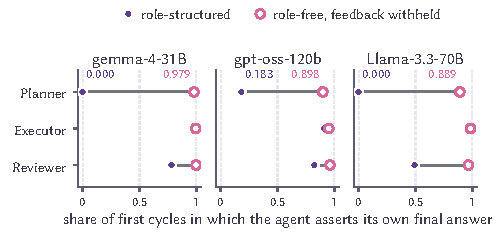
\includegraphics[width=\columnwidth]{figures/fig_supp_roles.pdf}
\Description{Three panels, one per actor. Each shows three horizontal
dumbbells, for the Planner, Executor and Reviewer, from the role-structured
value to the role-free value of the share of first cycles in which that
agent asserts its own final answer. The Planner's dumbbell spans almost the
whole axis in every panel; the Executor's is near one at both ends; the
Reviewer's is short.}
\caption{Which agent changes when the role clauses are deleted. For each
actor, the share of first cycles in which the Planner, Executor and
Reviewer assert their own final answer under role-structured prompts
(filled) and under role-free prompts with the evaluator's feedback withheld
(hollow), on the Omni-MATH benchmark. The Planner moves from almost never
answering to almost always answering; the Executor answers under both; the
Reviewer moves less.}
\label{fig:roles}
\end{figure}

\paragraph{The Planner is the agent that changes.} By role, the share of
first cycles in which an agent asserts its own final answer moves from RS
to RF$^{-}$ as follows, for gemma-4-31B-it, gpt-oss-120b and
Llama-3.3-70B-Instruct in turn: Planner $0.000$, $0.183$ and $0.000$ to
$0.979$, $0.898$ and $0.889$; Executor $0.973$, $0.907$ and $1.000$ to
$0.993$, $0.951$ and $0.982$; Reviewer $0.781$, $0.823$ and $0.492$ to
$0.998$, $0.961$ and $0.965$. The Executor's job is to produce the answer,
so it answers under both conditions. The Reviewer often states an answer
even with roles, plausibly because approving an answer tends to restate it.
The division of labor therefore rests on the Planner's single prohibition,
and the role-free footer, which asks every agent for its current answer,
lifts it.

\paragraph{The collapsed Planner redoes the Executor's work.} The numbers
in a Planner's first-cycle message and in the Executor's overlap more than
Planner and Executor messages from different problems in the same condition
do, by $+0.449$, $+0.680$ and $+0.432$ without roles against $+0.159$,
$+0.167$ and $+0.145$ with them (Jaccard similarity of the two number
sets). Under roles the Planner writes a plan and the Executor computes;
without them both compute the same quantities. The gpt-oss-120b value
without roles is not interpretable, because most of those Planner messages
are only a few characters long (the logging defect below).

\paragraph{A second opinion from a model judge.} A frontier model rated the
first cycles of $171$ sampled trajectories ($42$ RS, $56$ RF$^{-}$ and the
rest SE) against a rubric frozen before the first judgment, asking whether
a division of labor was realized. Its verdicts agree with the
functional-collapse measure (Table~\ref{tab:collapse_full}), and across the
three rubric questions checked for stability its repeated judgments agree
on $0.947$ to $0.959$ of the items. The judge did not see the grade, but it
could infer the condition, because role words were renamed rather than
equalized across conditions; the collapse claim therefore does not rest on
it.

\paragraph{The logging defect, in detail.} A message whose hidden reasoning
was discarded is short but slow, so we mark messages with fewer than $10$
visible characters per second of latency. They are $75.7\%$ of
gpt-oss-120b's role-free messages and $7.7\%$ of its role-structured ones,
and $93.4\%$ and $22.7\%$ of its first cycles contain at least one. The
runner's own fallback flag marks only $5.8\%$ and $2.7\%$ of the same
messages, which is why the defect was found late. For the other two actors
at most $0.5\%$ of messages are marked. The defect cannot have produced the
collapse: on first cycles with no marked message, gpt-oss-120b's functional
collapse is $0.821$ ($n=106$) without roles and $0.118$ ($n=1{,}236$) with
roles.

\paragraph{Validating the computation-abstention measure.} \Pone{}, the
pre-registered measure of whether a Planner abstains from computing, was
checked by hand on $72$ Planner messages against a definition frozen before
the adjudication sheet was opened, each judgment with a recorded reason. It
agrees with the hand labels on $0.903$ of messages (Cohen's $\kappa=0.806$;
precision $0.943$, recall $0.868$), clearing the pre-set $0.80$ threshold.
Agreement fell from $0.967$ at $n=30$ as adjudication continued, and we
report the final figure. Its residual errors point in opposite directions
(symbolic results with no digits are missed, restated givens are flagged),
so they do not push the measure one way.

\section{Recovery (R2)}
\label{sec:recovery}

The main paper reports that, given the same feedback, the role-free team
recovers more, and that against the feedback-withheld baseline the roles
look load-bearing. Table~\ref{tab:recovery} gives the frozen baseline
comparison on both populations, so the marginal rates and the paired test
can be checked against each other; the comparison with feedback is the main
paper's Table~2.

% ==========================================================================
% Table 2 (manuscript) -- first pass and recovery
%
% GENERATED FILE -- do not edit by hand. Any edit is overwritten.
% generating script : analysis/scripts/mk_tables.py
% canonical input   : analysis/out/FINAL_TABLES_OUTPUT.txt  sections T1, T3, T4
% frozen data       : experiments/results/FROZEN/, frozen_at 2026-09-30T10:09:30.201557
%                     11600 trajectories
%                     sha256 fa22a446d5314bb67b1c6a6444b511eeeae3eb8770419a36f182617eeccbf3b5  actor3.jsonl
%                     sha256 038e08aec4d4aee166106a6325309dfe2301faf339c7d0bf82338a74576424d4  armCp.jsonl
%                     sha256 e4e53cb117d91129991ce2fe87e336e152fc9ee6ca826d363f2bd5dd240d7130  campaign_v2.jsonl
% canonical-output sha256 : b26ccb5451a5eaed14046a27a980ba8797e5669912df907bc25f69bf60ad5b76
% generation date   : 2026-10-04  (derived from the canonical
%                     input's mtime, not wall-clock: regeneration must
%                     be byte-identical)
%
% EVERY figure names its population. The marginal and paired
% panels have DIFFERENT denominators and are not interchangeable;
% conflating them has already caused one error in this project.
% Recovery denominator = judged(r) and fp(r)==0: a recorded
% incorrect FIRST verdict, INCLUDING trajectories that later died
% in regeneration (STATISTICAL_AUDIT FATAL-1). Not graded(r).
% Significance is exact McNemar on discordant pairs, never a
% bootstrap CI bound (that label was seed-dependent).
%
% Reader-facing condition names per paper/TERMINOLOGY.md; internal arm
% codes are deliberately absent and their absence is asserted at
% generation time.
% ==========================================================================
\begin{table*}[t]
\centering
\caption{\textbf{First-pass accuracy and recovery, role-structured versus
role-free.} \textbf{The two panels have different denominators and must not
be read across.} \emph{Upper:} the marginal population --- every
trajectory in the cell, first pass over those receiving an evaluator verdict,
recovery over those whose \emph{first} verdict was incorrect
($n_{\mathrm{fpw}}$ in parentheses, computed per condition and therefore
\emph{not} a shared denominator). \emph{Lower:} the paired population
--- only problems first-pass wrong under \emph{both} conditions, one shared
denominator $n_{\mathrm{both}}$, which is the actual test. The recovery
denominator counts every trajectory with a recorded incorrect first verdict,
including those that later died in regeneration; these score $0$ under the
pre-registered rule. Pre-registered scoring throughout; $p$ is exact McNemar
on discordant pairs.}
\label{tab:recovery}
\small
\begin{tabular}{lcccccc}
\toprule
\multicolumn{7}{@{}l}{\emph{Marginal population} --- each condition on
its own denominator} \\
\midrule
 & \multicolumn{3}{c}{first pass}
 & \multicolumn{3}{c}{recovery $\mid$ first verdict wrong} \\
\cmidrule(lr){2-4}\cmidrule(lr){5-7}
actor & role-struct. & role-free & difference
      & role-struct. ($n$) & role-free ($n$) & difference \\
\midrule
gemma-4-31B & $0.802$ & $0.802$ & $+0.0000$ {\footnotesize $[{-}0.0156,\,+0.0150]$} & $0.222$ (316) & $0.051$ (316) & ${-}0.1709$ {\footnotesize $[{-}0.2247,\,{-}0.1171]$} \\
gpt-oss-120b & $0.713$ & $0.763$ & $+0.0503$ {\footnotesize $[+0.0339,\,+0.0666]$} & $0.324$ (463) & $0.247$ (380) & ${-}0.0766$ {\footnotesize $[{-}0.1361,\,{-}0.0153]$} \\
Llama-3.3-70B & $0.308$ & $0.316$ & $+0.0077$ {\footnotesize $[{-}0.0283,\,+0.0437]$} & $0.014$ (276) & $0.015$ (268) & $+0.0004$ {\footnotesize $[{-}0.0214,\,+0.0192]$} \\
\midrule
\multicolumn{7}{@{}l}{\emph{Paired population} --- problems first-pass
wrong under \textbf{both} conditions; one shared denominator} \\
\midrule
actor & $n_{\mathrm{both}}$ & role-struct. & role-free
      & role-struct.\ only & role-free only & exact $p$ \\
\midrule
gemma-4-31B & $237$ & $0.160$ & $0.017$ & $37$ & $3$ & $1.95\times 10^{-8}$ \\
gpt-oss-120b & $327$ & $0.242$ & $0.202$ & $52$ & $39$ & $0.208$ \\
Llama-3.3-70B & $245$ & $0.004$ & $0.016$ & $1$ & $4$ & $0.375$ \\
\bottomrule
\end{tabular}

\vspace{2pt}
\footnotesize Recovery conditions on a post-treatment variable and is
descriptive, never causal. No cell recovers before its first oracle verdict.
\end{table*}


\paragraph{Where the baseline gap comes from.} For gemma-4-31B-it the
accounting closes exactly. The two conditions reach a correct first answer
on the same number of problems ($1{,}284$ of $1{,}600$), and a correct first
answer is never lost because the loop halts on a PASS, so the gap in final
accuracy, $54$ problems in favor of roles ($p=1.6\times10^{-5}$), is exactly
the gap in recoveries, $70$ against $16$. Most of it arises on the $237$
problems both teams first miss, where $38$ are recovered with roles against
$4$ without; the problems that only one team first misses contribute a
further $20$ in the same direction. This accounting needs equal first-pass
counts and does not transfer to the other two actors.

\paragraph{The result reproduces.} The two gemma-4-31B-it cells of the RF
condition were run twice, independently and about thirteen hours apart,
with byte-identical runner and prompt code; every other RF cell was run
once. Table~\ref{tab:bfreplication} gives both runs against the frozen RS
cell. The ordering and the final-accuracy contrasts reproduce in both
domains; the SciBench paired recovery test, on $100$ problems, is $p=0.013$
in the first run and $p=0.052$ in the second, so on that benchmark the
recovery contrast is at the edge of resolution. Each run also repeated the
drift check of the main text on the same $400$ frozen problems: the RS
re-run reaches final accuracy $0.818$ in the first and $0.845$ in the
second, against $0.825$ frozen (paired $p=0.75$ and $p=0.20$). The main
text reports the first run throughout.

%% GENERATED by analysis/scripts/mk_bf_replication.py from FIGDATA_BF.json and
%% FIGDATA_BF_chain2.json -- do not edit by hand.
\begin{table*}[t]
\centering
\caption{\textbf{The gemma-4 feedback-matched cells, run twice.}
Role-structured: Planner, Executor and Reviewer prompts (the frozen run).
Role-free + feedback: one generic prompt for all three agents, with the
evaluator's verdict and repair hint shown; both runs use byte-identical
runner and prompt code, and the main text reports run 1. \emph{First
pass}: whether a trajectory's (one problem's run) first submitted answer is
correct. \emph{Recovery}: first-pass-wrong trajectories that finish
correct, over each condition's own first-pass-wrong set (count /
denominator). \emph{Final}: accuracy at the end over all problems,
never-graded trajectories counted as incorrect. The \emph{paired} columns
compare each role-free run with the role-structured run on problems
first-pass wrong under both (recovery) or on all problems (final): problems
recovered, or finally correct, only without roles versus only with them,
with the exact McNemar $p$ for the two counts.}
\label{tab:bfreplication}
\small
\begin{tabular}{@{}lccccc@{}}
\toprule
 & first pass & recovery & paired recovery & final & paired final \\
\midrule
\multicolumn{6}{@{}l}{\emph{Omni-MATH}} \\
\quad role-structured (frozen) & $0.802$ & $70/316=0.222$ & -- & $0.846$ & -- \\
\quad role-free + feedback, run 1 & $0.802$ & $193/317=0.609$ & $89$ vs $4$, $p=6.2\times10^{-22}$ & $0.921$ & $137$ vs $17$, $p=1.7\times10^{-24}$ \\
\quad role-free + feedback, run 2 & $0.811$ & $177/302=0.586$ & $95$ vs $7$, $p=7.8\times10^{-21}$ & $0.922$ & $139$ vs $18$, $p=2.4\times10^{-24}$ \\
\addlinespace
\multicolumn{6}{@{}l}{\emph{SciBench}} \\
\quad role-structured (frozen) & $0.794$ & $30/118=0.254$ & -- & $0.847$ & -- \\
\quad role-free + feedback, run 1 & $0.796$ & $49/117=0.419$ & $21$ vs $7$, $p=0.013$ & $0.880$ & $31$ vs $12$, $p=0.0054$ \\
\quad role-free + feedback, run 2 & $0.784$ & $54/124=0.435$ & $19$ vs $8$, $p=0.052$ & $0.878$ & $29$ vs $11$, $p=0.0064$ \\
\addlinespace
\bottomrule
\end{tabular}
\end{table*}


\paragraph{Recoveries are revisions, and the hints do not leak the answer.}
Of the $193$ recoveries of the gemma-4-31B-it RF team on Omni-MATH, $192$
pass with an answer different from the one first rejected ($541$ of $547$
across the five RF cells), so re-grading the same answer explains almost
none of them; identical evaluator prompts at temperature $0$ return
different verdicts in only $20$ of $2{,}790$ prompt groups ($0.0072$). The
evaluator writes each hint with the gold answer in view, so a hint could
hand the answer over. Hints contain it verbatim in at most $2.3\%$ of
failing verdicts in any cell, and dropping every gemma-4-31B-it Omni-MATH
trajectory that saw such a hint leaves recovery at $0.599$ for RF and
$0.212$ for RS, against $0.609$ and $0.222$ on all trajectories. We did not
audit partial leakage.

\section{The submission gate (R3)}
\label{sec:gate}

The main paper's account of what roles do after feedback is that the
role-structured Reviewer gates submission: the RS team asks for fewer
verdicts, and matched on verdicts the two teams recover alike. This section
gives the evidence in three steps: where the declines happen
(Table~\ref{tab:gate}), how recovery tracks exposure to the evaluator
(Figure~\ref{fig:verdicts}), and how far the verdict-matched comparison can
be pushed (Table~\ref{tab:robust}, Figure~\ref{fig:robustness}a). The
forced-submission run (Table~\ref{tab:forced}) then removes the gate
directly.

%% GENERATED by analysis/scripts/mk_gate_table.py from FIGDATA_GATE.json and
%% FIGDATA_BF.json -- do not edit by hand.
\begin{table*}[t]
\centering
\caption{\textbf{Where the role-structured Reviewer declines, and what each
allocation buys.} RS: role-structured (Planner, Executor and Reviewer
prompts); RF: role-free (one generic prompt for all three agents) with the
evaluator's feedback shown. Every column is over first-pass-wrong
trajectories (one problem's run whose first submitted answer was graded
wrong), per actor (the model playing all three agents) and benchmark. A
cycle is one pass of the three agents; it ends in a submission to the
evaluator when the third agent approves and in a decline otherwise.
\emph{RS declining cycles} per trajectory, split into those before the
first submission (no feedback yet), those in a cycle that received a FAIL
verdict (where the role-structured clause forbids approval) and the
remaining ``free'' cycles; \emph{clause share} is the FAIL column as a
fraction of all three. \emph{RS never submits}: trajectories with no
approval in six cycles, graded once at the end. \emph{Free-cycle approval}:
the share of free cycles ending in approval. \emph{By 2nd verdict}: the
share recovered (finishing correct) with at most one round of feedback,
over all first-pass-wrong trajectories. \emph{Per later verdict}:
recoveries per verdict after the first, a ratio over different trajectories
in the two conditions (the verdict-matched comparison of the main paper's
Table~2 is the like-for-like one). \emph{Approvals}: submissions per
trajectory.}
\label{tab:gate}
\footnotesize
\setlength{\tabcolsep}{3.0pt}
\begin{tabular}{@{}l ccc c c cc cc cc cc@{}}
\toprule
 & \multicolumn{3}{c}{RS declining cycles} & clause & RS never
 & \multicolumn{2}{c}{free-cycle approval} & \multicolumn{2}{c}{by 2nd verdict}
 & \multicolumn{2}{c}{per later verdict} & \multicolumn{2}{c}{approvals} \\
\cmidrule(lr){2-4}\cmidrule(lr){7-8}\cmidrule(lr){9-10}\cmidrule(lr){11-12}\cmidrule(lr){13-14}
actor, domain & before & FAIL & free & share & submits & RS & RF & RS & RF & RS & RF & RS & RF \\
\midrule
gemma-4, Omni-MATH & $2.24$ & $0.81$ & $1.20$ & $0.19$ & $84/316$ & $0.25$ & $0.96$ & $0.206$ & $0.438$ & $0.41$ & $0.28$ & $1.27$ & $3.20$ \\
gpt-oss, Omni-MATH & $1.33$ & $1.17$ & $0.71$ & $0.37$ & $51/463$ & $0.53$ & $0.68$ & $0.246$ & $0.296$ & $0.27$ & $0.22$ & $2.10$ & $3.53$ \\
Llama-3.3, Omni-MATH & $4.49$ & $0.25$ & $0.88$ & $0.04$ & $205/276$ & $0.01$ & $0.82$ & $0.014$ & $0.092$ & $0.25$ & $0.08$ & $0.32$ & $2.71$ \\
gemma-4, SciBench & $0.55$ & $1.38$ & $1.48$ & $0.40$ & $3/118$ & $0.35$ & $0.99$ & $0.237$ & $0.239$ & $0.26$ & $0.16$ & $1.95$ & $3.62$ \\
gpt-oss, SciBench & $0.41$ & $1.53$ & $0.60$ & $0.60$ & $1/124$ & $0.67$ & $0.78$ & $0.258$ & $0.317$ & $0.19$ & $0.16$ & $2.68$ & $3.95$ \\
\bottomrule
\end{tabular}
\end{table*}


\paragraph{Where the Reviewer declines.} On Omni-MATH the clause that
forbids approval after a FAIL covers only a minority of the RS Reviewer's
declines, between $4\%$ and $37\%$ depending on the actor, and in the free
cycles, where no clause applies, it approves far less often than the RF
team's third agent (Table~\ref{tab:gate}). The gate is therefore mostly the
Reviewer's disposition rather than the letter of its prompt; gpt-oss-120b's
Reviewer is the most permissive of the three. On SciBench the clause covers
more of the declines, and the RS team almost always submits at least once,
which is why the recovery contrast is weaker there (Section~\ref{sec:xdomain}).

\begin{figure*}[t]
\centering
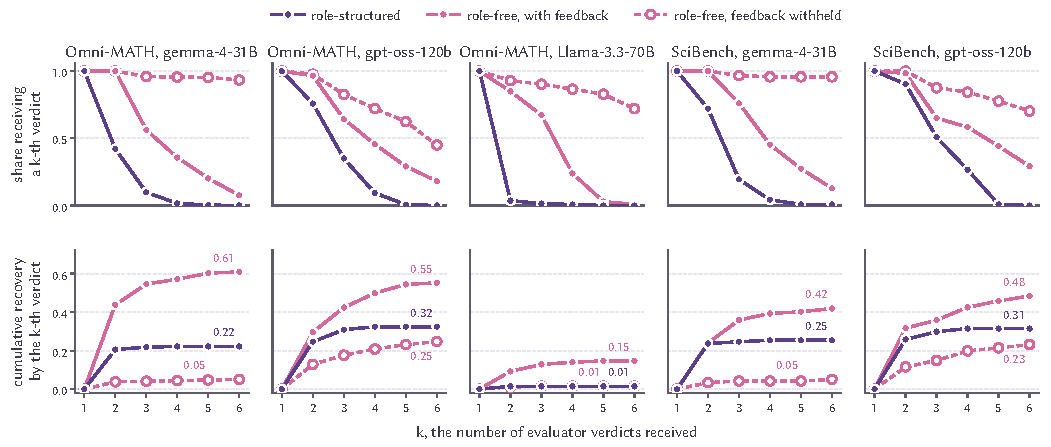
\includegraphics[width=\textwidth]{figures/fig_supp_verdicts.pdf}
\Description{Two rows of five panels, one column per cell. Top row: the
share of first-pass-wrong trajectories that receive a k-th verdict, falling
steeply for the role-structured team, more slowly for the role-free team
with feedback, and hardly at all for the role-free team without feedback.
Bottom row: cumulative recovery by the k-th verdict; the role-structured
curve flattens after the second verdict while the role-free curve with
feedback keeps rising.}
\caption{Recovery follows exposure to the evaluator. Top: the share of
first-pass-wrong trajectories that receive a $k$-th evaluator verdict.
Bottom: the cumulative share recovered by the $k$-th verdict, with the
final value labeled. One panel per cell (actor on benchmark):
role-structured (purple), role-free with feedback (rose) and role-free with
the feedback withheld (hollow, dashed). The role-structured curve flattens
where its trajectories stop receiving verdicts, not where they stop using
them.}
\label{fig:verdicts}
\end{figure*}

\paragraph{Recovery tracks exposure.} Figure~\ref{fig:verdicts} shows the
mechanism directly. In every cell the RS team's share of trajectories still
receiving verdicts falls steeply after the first one, while the RF team's
falls slowly, and the cumulative recovery curves follow the exposure
curves. Per verdict received, the two teams recover alike: on the paired
problems, pooled over the five cells, the share whose second verdict is a
PASS is $0.267$ for RS and $0.224$ for RF, and at the third and fourth
verdicts $0.083$ against $0.127$ and $0.105$ against $0.089$. Recoveries
per verdict after the first are higher with roles in every cell
(Table~\ref{tab:gate}), but that ratio compares different trajectories,
since most of the RF team's later verdicts are further attempts on problems
it has already failed more than once; the like-for-like comparison is the
verdict-matched one.

\paragraph{How far the verdict-matched comparison can be pushed.} Matching
on verdicts is coarse. When the RS team received a single verdict, because
it never submitted and was graded at the end or because it submitted once
and stopped, the RF trajectory cut to one verdict cannot recover either,
and the pair ties at zero by construction. These forced ties are most of
the gemma-4-31B-it pairs and nearly all of the Llama-3.3-70B-Instruct pairs
(Table~\ref{tab:robust}), so the pooled interval of the main paper is
narrower than the information behind it. The cut is also one-sided, since
the RS count stops at that team's own passing verdict, which can only favor
it. Table~\ref{tab:robust} and Figure~\ref{fig:robustness}a therefore give
the contrast under six definitions: the problems with at least two RS
verdicts, both trajectories cut at the smaller count, and the scoring
defect recoded, each with and without Llama-3.3-70B-Instruct. No variant
puts the RF team significantly ahead: the two symmetric cuts favor it by
$0.005$ and $0.010$ with intervals that include zero, the informative
problems allow up to $+0.065$ in favor of roles ($+0.073$ with the
recoding), and with the recoding on all problems the RS team leads by
$+0.029$ with an interval that excludes zero. The defensible reading is the
main paper's: matched on verdicts the RF advantage disappears, and any
per-verdict advantage of roles is small. Matching equalizes exposure to the
evaluator, not calls; the RS team spends more cycles per verdict.

%% GENERATED by analysis/scripts/mk_robust_table.py from FIGDATA_GATE.json
%% (bf_gate.py [G4], [G6]) -- do not edit by hand.
\begin{table*}[t]
\centering
\caption{\textbf{Robustness of the verdict-matched recovery contrast.} RS:
role-structured (Planner, Executor and Reviewer prompts); RF: role-free
(one generic prompt for all three agents) with the evaluator's feedback
shown; a cell is one actor (the model playing all three agents) on one
benchmark. The contrast takes the problems both teams first answer wrongly
and cuts the RF trajectory (one problem's run) after as many evaluator
verdicts (PASS or FAIL decisions) as the RS trajectory received on that
problem, then compares recovery (finishing correct). Where RS received a
single verdict (it never submitted again, or submitted once and stopped),
the cut RF trajectory cannot recover either, so the pair ties at zero by
construction. \emph{Upper block}: such forced ties per cell, how many of
them never submitted, the problems left, and the trajectories whose held
answer matched the key but were graded wrong (the scoring defect of the
main paper's Limitations). \emph{Middle block}: the pooled difference (RS
minus RF, stratified by cell, $95\%$ bootstrap confidence interval
resampling problems) under six definitions, with and without Llama-3.3;
\emph{equivalent} means the $90\%$ interval lies inside $\pm0.05$. Recoding
counts an RS trajectory with a correct held answer as recovered, and an RF
one only if it was not cut. \emph{Lower block}: per-verdict pass rates, the
share of trajectories whose $k$-th verdict is PASS among those whose
earlier verdicts all failed, pooled over the five cells.}
\label{tab:robust}
\footnotesize
\begin{tabular}{@{}l ccccc@{}}
\toprule
cell & paired $n$ & forced ties & never submitted & left & held-answer recodes (RS / RF) \\
\midrule
gemma-4, Omni-MATH & $236$ & $141$ & $66$ & $95$ & $12$ / $3$ \\
gpt-oss, Omni-MATH & $319$ & $84$ & $36$ & $235$ & $4$ / $0$ \\
Llama-3.3, Omni-MATH & $250$ & $242$ & $187$ & $8$ & $2$ / $1$ \\
gemma-4, SciBench & $100$ & $29$ & $2$ & $71$ & $2$ / $0$ \\
gpt-oss, SciBench & $93$ & $11$ & $1$ & $82$ & $0$ / $0$ \\
\bottomrule
\end{tabular}

\vspace{4pt}
\begin{tabular}{@{}l c l c c l@{}}
\toprule
 & \multicolumn{3}{c}{all five cells} & \multicolumn{2}{c}{without Llama-3.3} \\
\cmidrule(lr){2-4}\cmidrule(lr){5-6}
definition & $n$ & difference [95\% CI] & equivalent & $n$ & difference [95\% CI] \\
\midrule
as in Table~2 & $998$ & $+0.009$ {\footnotesize $[{-}0.014,\,+0.033]$} & yes & $748$ & $+0.011$ {\footnotesize $[{-}0.020,\,+0.043]$} \\
role-structured team received $\geq2$ verdicts & $491$ & $+0.018$ {\footnotesize $[{-}0.029,\,+0.065]$} & no & $483$ & $+0.017$ {\footnotesize $[{-}0.031,\,+0.064]$} \\
both cut at the smaller verdict count & $998$ & ${-}0.005$ {\footnotesize $[{-}0.029,\,+0.019]$} & yes & $748$ & ${-}0.008$ {\footnotesize $[{-}0.040,\,+0.024]$} \\
both cut, $\geq2$ verdicts & $491$ & ${-}0.010$ {\footnotesize $[{-}0.059,\,+0.039]$} & no & $483$ & ${-}0.012$ {\footnotesize $[{-}0.062,\,+0.037]$} \\
scoring defect recoded & $998$ & $+0.029$ {\footnotesize $[+0.004,\,+0.054]$} & no & $748$ & $+0.035$ {\footnotesize $[+0.003,\,+0.067]$} \\
recoded, $\geq2$ verdicts & $491$ & $+0.026$ {\footnotesize $[{-}0.020,\,+0.073]$} & no & $483$ & $+0.025$ {\footnotesize $[{-}0.023,\,+0.072]$} \\
\bottomrule
\end{tabular}

\vspace{4pt}
\begin{tabular}{@{}l cc@{}}
\toprule
per-verdict pass rate & role-structured & role-free with feedback \\
\midrule
verdict 2 & $131/491=0.267$ & $212/946=0.224$ \\
verdict 3 & $19/228=0.083$ & $89/700=0.127$ \\
verdict 4 & $8/76=0.105$ & $39/439=0.089$ \\
\bottomrule
\end{tabular}
\end{table*}


\begin{figure*}[t]
\centering
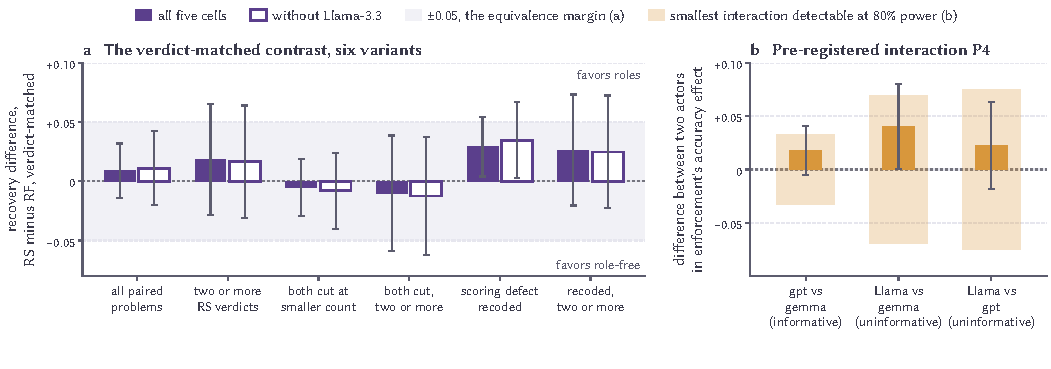
\includegraphics[width=\textwidth]{figures/fig_supp_robustness.pdf}
\Description{Two bar charts with error bars. Left: six pairs of bars,
one pair per definition of the verdict-matched contrast, all small and
with intervals that cross or nearly cross zero, inside a shaded band from
minus 0.05 to plus 0.05. Right: three bars for the pre-registered
interaction, each with an interval, drawn over a wider shaded bar showing
the smallest detectable effect; for two of the three the shaded bar is
wider than the band.}
\caption{Two robustness checks. (a) The verdict-matched recovery
difference, role-structured minus role-free with feedback, pooled over the
five cells (filled) and without Llama-3.3-70B-Instruct (hollow), under the
six definitions of Table~\ref{tab:robust}, with $95\%$ intervals; the band
marks the $\pm0.05$ equivalence margin. (b) The pre-registered interaction
P4 (Section~\ref{sec:prereg}): each difference between two actors in
enforcement's effect on final accuracy, with its $95\%$ interval; the
shaded bar behind it spans the smallest interaction detectable at $80\%$
power. Where that bar is wider than any plausible effect, the null is
uninformative.}
\label{fig:robustness}
\end{figure*}

\paragraph{Across the freeze.} The frozen RS cell and the RF team were run
on opposite sides of the freeze, so we repeat the comparison against the
post-freeze RS re-run of gemma-4-31B-it on $400$ Omni-MATH problems. On the
$65$ problems both first answer wrongly, the RF team leads $22$ to $3$
unmatched ($p=1.6\times10^{-4}$), but the RS team leads $4$ to $1$
verdict-matched ($p=0.38$): the same pattern as in the frozen comparison.

\paragraph{Removing the gate alone.} The forced-submission run tests the
gate directly. It uses the RS prompts and runner unchanged except for one
step: after the Reviewer's turn, the pipeline submits the team's current
answer to the evaluator whatever route the Reviewer chose, and the verdict
and hint reach the agents through the same role-specific slots as in the RS
condition. An offline test in the supplementary material (no model calls)
checks that the prompts are byte-identical to the RS ones up to the first
verdict and that the evaluator is called in every cycle. It was run once,
after the freeze, for gemma-4-31B-it on the $400$ Omni-MATH problems of the
RS re-run, with the same server, budget and evaluator.
Table~\ref{tab:forced} compares it with that re-run, the frozen RS cell and
the RF team, restricted to the same problems. Recovery rises to the RF
team's level while first-pass accuracy does not move: once the Reviewer's
approvals no longer decide anything, the role prompts recover as much as
the generic ones.

%% GENERATED by analysis/scripts/mk_afs_table.py from FIGDATA_GATE.json
%% (bf_gate.py [G5]) -- do not edit by hand.
\begin{table*}[t]
\centering
\caption{\textbf{Removing the submission gate.} gemma-4, Omni-MATH, the
same $400$ problems in every row. The forced-submission run uses the
role-structured prompts byte for byte; the pipeline submits the team's answer
to the evaluator in every cycle, whatever the Reviewer decides. Recovery is
over each row's own first-pass-wrong trajectories; verdicts and Reviewer
approvals are per first-pass-wrong trajectory and include the first. In the
forced-submission run approvals are logged but do not decide submission. The
lower block pairs the conditions on the problems both first answer wrongly
(recovery) and on all problems (final accuracy): problems solved only by the
first condition / only by the second, exact McNemar $p$.}
\label{tab:forced}
\footnotesize
\begin{tabular}{@{}l ccccc@{}}
\toprule
condition & first pass & recovery & final accuracy & verdicts & Reviewer approvals \\
\midrule
role-structured, every cycle submitted & $0.767$ & $57/93=0.613$ & $0.910$ & $4.20$ & $0.98$ \\
role-structured, re-run after the freeze & $0.772$ & $18/91=0.198$ & $0.818$ & $1.44$ & $1.13$ \\
role-structured, frozen snapshot & $0.795$ & $12/82=0.146$ & $0.825$ & $1.41$ & $1.15$ \\
role-free with feedback & $0.795$ & $45/82=0.549$ & $0.907$ & $3.34$ & $3.34$ \\
\bottomrule
\end{tabular}

\vspace{4pt}
\begin{tabular}{@{}l ccc cc@{}}
\toprule
 & \multicolumn{3}{c}{recovery (both first wrong)} & \multicolumn{2}{c}{final accuracy} \\
\cmidrule(lr){2-4}\cmidrule(lr){5-6}
pair & $n$ & first / second only & $p$ & first / second only & $p$ \\
\midrule
every cycle submitted vs.\ re-run & $72$ & $26$ / $2$ & $3.0{\times}10^{-6}$ & $42$ / $5$ & $2.5{\times}10^{-8}$ \\
every cycle submitted vs.\ role-free with feedback & $70$ & $7$ / $7$ & $1$ & $8$ / $7$ & $1$ \\
re-run vs.\ role-free with feedback & $65$ & $3$ / $22$ & $1.6{\times}10^{-4}$ & $6$ / $42$ & $1.0{\times}10^{-7}$ \\
\bottomrule
\end{tabular}
\end{table*}


\section{The second domain (R4)}
\label{sec:xdomain}

Table~\ref{tab:scibench} is the SciBench replication in full: the frozen
comparison with its denominators, for the two actors run there. The main
paper carries both actors in its Figure~2 and Table~2.

% ==========================================================================
% Table 3 (manuscript) -- SciBench cross-domain replication
%
% GENERATED FILE -- do not edit by hand. Any edit is overwritten.
% generating script : analysis/scripts/mk_tables.py
% canonical input   : analysis/scripts/xdom_analyze.py (executed; stdout parsed)
%                      which execs FINAL_TABLES.py and rebinds its definitions
%                      -- judged / is_fpw / fp / fin_prereg are the SAME code
%                      objects as the Omni-MATH tables, not a reimplementation
% frozen data       : experiments/results/FROZEN/, frozen_at 2026-09-30T10:09:30.201557
%                     11600 trajectories
%                     sha256 fa22a446d5314bb67b1c6a6444b511eeeae3eb8770419a36f182617eeccbf3b5  actor3.jsonl
%                     sha256 038e08aec4d4aee166106a6325309dfe2301faf339c7d0bf82338a74576424d4  armCp.jsonl
%                     sha256 e4e53cb117d91129991ce2fe87e336e152fc9ee6ca826d363f2bd5dd240d7130  campaign_v2.jsonl
% canonical-output sha256 : 4f157fe9ff37c759844393e8af22c61e5b14875a98e4dee870a1a57c5451f036
% generation date   : 2026-10-01  (derived from the canonical
%                     input's mtime, not wall-clock: regeneration must
%                     be byte-identical)
%
% SciBench frozen data: experiments/results/xdomain/FROZEN_SCIBENCH/
%   frozen_at 2026-09-30T23:26:47.198588+00:00, 2296 trajectories
%   sha256 10068f72cfd936d3be6de85fef196d63fc154ef2c2ec26a0ac2c7313513dce58  scibench_AB.jsonl
% gpt-oss's recovery cell is UNDERPOWERED, not a non-replication:
% its point estimate matches Omni-MATH's. Llama-3.3 was not run.
% No clause-specific role-fidelity metric crosses domains (the
% contract was domain-adapted), so none is reported here.
%
% Reader-facing condition names per paper/TERMINOLOGY.md; internal arm
% codes are deliberately absent and their absence is asserted at
% generation time.
% ==========================================================================
\begin{table*}[t]
\centering
\caption{\textbf{The dissociation replicates out of domain.} SciBench,
the complete $574$-problem matched slice of free-response college science;
two actors, 2296 trajectories, frozen separately from the
Omni-MATH snapshot. \textbf{The two panels have different populations.}
First pass is paired over all $574$ problems; paired recovery is over only
those first-pass wrong under \emph{both} conditions
($n_{\mathrm{both}}$), which is why its $n$ is roughly a sixth the size.
Pre-registered scoring; $p$ is exact McNemar on discordant pairs. gpt-oss's
recovery cell \textbf{cannot resolve its own effect} at the realized
$n_{\mathrm{both}}$ --- its point estimate is in the same direction and
nearly the same size as Omni-MATH's, so it is underpowered rather than a
non-replication. Llama-3.3 was not run in this domain.}
\label{tab:scibench}
\small
\begin{tabular}{lccccc@{\hspace{1.4em}}ccccccc}
\toprule
 & \multicolumn{5}{c}{first pass (paired, all problems)}
 & \multicolumn{7}{c}{recovery (paired on first-pass wrong under both)} \\
\cmidrule(lr){2-6}\cmidrule(lr){7-13}
actor & $n$ & role-str. & role-free & diff. & exact $p$
      & $n_{\mathrm{both}}$ & role-str. & role-free & diff.
      & r-s.\ only & r-f.\ only & exact $p$ \\
\midrule
gemma-4-31B & $574$ & $0.794$ & $0.794$ & $+0.0000$ & $1.00\times 10^{0}$ & $99$ & $0.212$ & $0.020$ & ${-}0.1919$ & $21$ & $2$ & $6.60\times 10^{-5}$ \\
gpt-oss-120b & $574$ & $0.784$ & $0.789$ & $+0.0052$ & $0.784$ & $96$ & $0.219$ & $0.135$ & ${-}0.0833$ & $17$ & $9$ & $0.169$ \\
\bottomrule
\end{tabular}
\end{table*}


\paragraph{What was and was not changed.} The prompts are not byte-identical
to Omni-MATH's, and the prompt files in the supplementary material make the
difference checkable. Of the $16$ prompts the two domains share, $11$ are
identical and $5$ differ: four of the six RS prompts (the Planner, Executor
and Reviewer preambles and the Reviewer's routing rules) and the evaluator's
preamble, which must ask for scientific rather than mathematical
equivalence. Both RF prompts are identical across domains, as are the six SE
prompts (enforcement was not run on SciBench). The asymmetry deserves
stating plainly: the RS prompts, whose team recovers less than the RF team,
are the ones that were rewritten, while the RF prompts ran identical text in
both domains. The rewrite is domain wording (``algebraic manipulation or
numerical calculation'' where Omni-MATH said ``symbolic manipulation or
arithmetic''), and the structural clauses are unchanged; a reader who
suspects the adaptation is doing the work can check the files. Topology,
budget, decoding, retry policy and the evaluator protocol are unchanged, so
this is a replication of the mechanism under a matched protocol, not a
rerun of identical prompts.

\paragraph{Why the answer does not lock here.} On Omni-MATH the
gemma-4-31B-it RS team often keeps the same answer across cycles (a single
distinct answer in $28.8\%$ of its failed trajectories); on SciBench it does
not ($7.6\%$, against $8.5\%$ for the RF team). The RS team on SciBench also
almost always submits at least once (Table~\ref{tab:gate}), so it sees more
feedback, and by the second verdict the two teams recover alike. A looser
gate is the simplest common explanation of both observations, though we did
not test it.

\section{Structural enforcement (R5)}
\label{sec:enforcement}

The main paper reports that enforcement loosens the gate and raises
revisability, but that attrition keeps the gain from reaching end-to-end
accuracy, and that the apparent accuracy benefit under the as-graded scoring
is survivorship. Table~\ref{tab:enforcement} and
Figure~\ref{fig:enforcement} are the evidence for both halves: the
manipulation check, the one-sided attrition, and the same accuracy
difference under both scorings.

% ==========================================================================
% Table 4 (manuscript) -- structural enforcement
%
% GENERATED FILE -- do not edit by hand. Any edit is overwritten.
% generating script : analysis/scripts/mk_tables.py
% canonical input   : analysis/out/FINAL_TABLES_OUTPUT.txt  sections T1, T2, T7, T11
% frozen data       : experiments/results/FROZEN/, frozen_at 2026-09-30T10:09:30.201557
%                     11600 trajectories
%                     sha256 fa22a446d5314bb67b1c6a6444b511eeeae3eb8770419a36f182617eeccbf3b5  actor3.jsonl
%                     sha256 038e08aec4d4aee166106a6325309dfe2301faf339c7d0bf82338a74576424d4  armCp.jsonl
%                     sha256 e4e53cb117d91129991ce2fe87e336e152fc9ee6ca826d363f2bd5dd240d7130  campaign_v2.jsonl
% canonical-output sha256 : b26ccb5451a5eaed14046a27a980ba8797e5669912df907bc25f69bf60ad5b76
% generation date   : 2026-10-04  (derived from the canonical
%                     input's mtime, not wall-clock: regeneration must
%                     be byte-identical)
%
% The manipulation-check column is ANSWER AUTHORSHIP = 1 minus
% T11's 'authored-free' column, which is a FREEDOM rate. The
% manuscript once read that axis inverted (APPROVED_CLAIMS A11);
% the complement is taken here, once, in code.
% Recovery denominator as in Table 2 (judged & fp==0).
% APPROVED_CLAIMS A6: enforcement restores recovery for Llama-3.3
% ONLY. For the other two the direction is consistent but not
% resolvable. 'Highest of any arm, above role-structured in all
% three actors' is a DEAD claim and must not reappear.
% The as-graded column is SENSITIVITY ONLY -- it is the
% survivorship reading, which is why attrition sits beside it.
%
% Reader-facing condition names per paper/TERMINOLOGY.md; internal arm
% codes are deliberately absent and their absence is asserted at
% generation time.
% ==========================================================================
\begin{table*}[t]
\centering
\caption{\textbf{Structural enforcement.} Enforcing the division of labor
at the interface. \emph{Manipulation check:} the rate at which the planner
authors an answer, over all planner messages, under enforcement and (in
parentheses) when roles are merely deleted --- enforcement drives it to zero
in all three actors, so the intervention engaged (the main paper's R5 gives
the first-pass rate). \emph{Locked answer:} the team never changed its
answer string, among first-pass-wrong trajectories (role-free, feedback
withheld / role-structured in parentheses). \emph{Recovery:} role-structured in parentheses, on the
denominator of Table~\ref{tab:recovery}. \textbf{The two accuracy columns
are different populations, and the attrition column is why they disagree.}
The pre-registered rule scores never-graded trajectories incorrect; the
as-graded column drops them and is a \emph{sensitivity analysis only} ---
its gains are conditional on parsing successfully, and enforcement is the
only condition where that removes a material fraction of the data.
\textbf{Enforcement restores recovery for Llama-3.3; for the other two
actors the direction is consistent but not resolvable against that
attrition.}}
\label{tab:enforcement}
\small
\begin{tabular}{lccccccc}
\toprule
 & planner authors & locked answer & recovery & &
 \multicolumn{2}{c}{final accuracy, enforced $-$ role-structured} \\
\cmidrule(lr){6-7}
actor & answer (role-free) & (r-f./r-s.) & (role-str.) & attrition
      & pre-registered & as-graded \\
 & \footnotesize manipulation check & \footnotesize first-pass wrong
 & \footnotesize first-pass wrong & & \footnotesize (primary)
 & \footnotesize (sensitivity) \\
\midrule
gemma-4-31B & $0.000$ (0.986) & $0.119$ (0.845/0.288) & $0.314$ (0.222) & $8.0\%$ & ${-}0.0225$ {\footnotesize [-0.0387,-0.0063]} & $+0.0190$ {\footnotesize [+0.0054,+0.0333]} \\
gpt-oss-120b & $0.000$ (0.916) & $0.092$ (0.208/0.052) & $0.395$ (0.324) & $9.9\%$ & ${-}0.0050$ {\footnotesize [-0.0219,+0.0112]} & $+0.0361$ {\footnotesize [+0.0215,+0.0507]} \\
Llama-3.3-70B & $0.000$ (0.958) & $0.072$ (0.806/0.750) & $0.139$ (0.014) & $17.0\%$ & $+0.0175$ {\footnotesize [-0.0200,+0.0550]} & $+0.0453$ {\footnotesize [+0.0030,+0.0876]} \\
\bottomrule
\end{tabular}

\vspace{2pt}
\footnotesize Attrition elsewhere is negligible: $0.0$--$0.8\%$ with roles,
$0.0$--$2.5\%$ without. The as-graded column turns every sign
positive; the pre-registration fixed in advance that unparseable
trajectories count incorrect, and \textbf{the benefit appears only after
conditioning on successful parsing.}
\end{table*}


\begin{figure}[t]
\centering
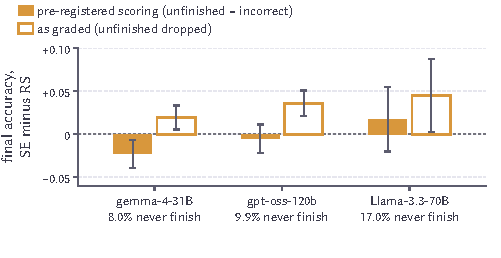
\includegraphics[width=\columnwidth]{figures/fig_supp_enforcement.pdf}
\Description{A bar chart with error bars. For each of three actors, two
bars of the accuracy difference between the enforced and the
role-structured condition, one under the pre-registered scoring and one as
graded; the as-graded bar is higher than the pre-registered one in every
group. The tick labels give each actor's share of enforced trajectories
that never finish, from 8 percent to 17 percent.}
\caption{Enforcement's effect on final accuracy under the two scorings.
Enforced minus role-structured final accuracy per actor with $95\%$
intervals, under the pre-registered scoring (unfinished trajectories count
as incorrect; filled) and as graded (they are dropped; hollow). The tick
labels give the share of enforced trajectories that never finish, which is
what separates the two bars. The sign flips between the scorings for two
of the three actors, and the as-graded gains are ordered like the
attrition.}
\label{fig:enforcement}
\end{figure}

\paragraph{Why the columns do not compose.} The enforced recovery and
first-pass rates do not combine into the accuracy column, and cannot:
trajectories that never receive a first verdict have no first pass, and
those that die after one stay in the recovery denominator, so the three
quantities do not share a denominator. The pre-registration fixed in advance
that unparseable trajectories count as incorrect rather than being dropped,
and that rule is what makes the as-graded reading survivorship rather than a
finding.

\paragraph{The gate loosens, and brittleness follows the same order.} Per
failed trajectory, the SE Reviewer approves $2.02$, $2.33$ and $1.84$ times
for gemma-4-31B-it, gpt-oss-120b and Llama-3.3-70B-Instruct, against
$1.27$, $2.10$ and $0.32$ under RS prompts. Enforcement logs $838$,
$1{,}183$ and $395$ role-boundary rejections, that is $0.52$, $0.74$ and
$0.99$ per trajectory, in the same order as the attrition ($8.0\%$, $9.9\%$
and $17.0\%$): the actor that breaks the schema most often is the one that
loses the most trajectories. For Llama-3.3-70B-Instruct, whose RS team
rarely submits, enforced recovery comes close to the RF team's ($0.139$
against $0.147$); on the $219$ problems both first answer wrongly, $9$ are
recovered only under enforcement and $17$ only by the RF team ($p=0.17$).

\paragraph{The context-restored control.} Enforcement also hides the
shared history from the Executor, so part of its brittleness may be lost
context rather than the typed interface. Restoring the shared history
at fixed enforcement (gemma-4-31B-it and gpt-oss-120b, $400$ problems each;
attrition $4.5\%$ and $9.8\%$) changes final accuracy relative to
enforcement by $+0.0450$ $[+0.0125,+0.0775]$ ($p=0.0079$) for gemma-4-31B-it
and by $-0.0125$ $[-0.0475,+0.0200]$ ($p=0.56$) for gpt-oss-120b under the
pre-registered scoring, and by $+0.0196$ $[-0.0028,+0.0419]$ ($p=0.14$) and
$-0.0089$ $[-0.0357,+0.0149]$ ($p=0.65$) as graded. For gemma-4-31B-it the
gain is significant only under the scoring that penalizes attrition, so it
comes mostly from fewer trajectories dying; the control is partial, because
the attrition it removes is one-sided.

% ==========================================================================
% Table 6 (supplement) -- pre-registered endpoints
%
% GENERATED FILE -- do not edit by hand. Any edit is overwritten.
% generating script : analysis/scripts/mk_tables.py
% canonical input   : analysis/out/FINAL_TABLES_OUTPUT.txt  sections T2, T14, T29
%                    analysis/scripts/stat_audit_a7_power.py (executed) -- MDE only
% frozen data       : experiments/results/FROZEN/, frozen_at 2026-09-30T10:09:30.201557
%                     11600 trajectories
%                     sha256 fa22a446d5314bb67b1c6a6444b511eeeae3eb8770419a36f182617eeccbf3b5  actor3.jsonl
%                     sha256 038e08aec4d4aee166106a6325309dfe2301faf339c7d0bf82338a74576424d4  armCp.jsonl
%                     sha256 e4e53cb117d91129991ce2fe87e336e152fc9ee6ca826d363f2bd5dd240d7130  campaign_v2.jsonl
% canonical-output sha256 : 4f157fe9ff37c759844393e8af22c61e5b14875a98e4dee870a1a57c5451f036
% generation date   : 2026-10-01  (derived from the canonical
%                     input's mtime, not wall-clock: regeneration must
%                     be byte-identical)
%
% P4 -- THE pre-registered primary -- is NULL before and after
% Holm. Reported as the failure of the thesis it was written to
% test (APPROVED_CLAIMS A10).
% P1 FAILED AS WRITTEN and was re-designated: the schema forbids
% emitting an ANSWER, not performing COMPUTATION. Reported as a
% finding, not hidden (DECISION_LOG D9/R1).
% P2 and P5 yield no p-value and are not p-corrected; the Holm
% family is therefore P3's three contrasts and P4's three DiDs,
% which is what the canonical output corrects.
% 
% PREREG_MDE_POPULATION_NOTE -- the MDE column and the
% difference-in-difference column come from DIFFERENT
% populations and are not arithmetically consistent:
%   * T14's DiD differences two per-actor C-A means computed on
%     each actor's OWN problem set (n=1600 and n=400).
%   * the MDE is computed on problems shared by BOTH actors,
%     where the Llama/gemma-4 observed DiD is +0.0300, not the
%     +0.0400 T14 prints.
% Both are correct for their own question; the MDE is quoted only
% as a detectability scale, never as the effect estimate. Do not
% recompute one from the other.
%
% Reader-facing condition names per paper/TERMINOLOGY.md; internal arm
% codes are deliberately absent and their absence is asserted at
% generation time.
% ==========================================================================
\begin{table*}[t]
\centering
\caption{\textbf{Every pre-registered endpoint, and what became of it.}
Fixed in writing before any intervention data existed. \textbf{P4 --- the
pre-registered primary test --- is null, before and after the pre-registered
Holm correction}, and we report it as the failure of the thesis it was
written to test. P1 failed \emph{as written} and was re-designated rather
than dropped: the interface forbids the planner emitting an \emph{answer},
and nothing in it stops the planner \emph{computing} --- a dissociation we
report as a finding. P2 and P5 are reported as effects and associations and
carry no $p$-value, so the correctable family is P3's three contrasts and
P4's three difference-in-differences. \textbf{The MDE column is a
detectability scale on a different population from the effect column} ---
it is computed on problems shared by both actors, while each
difference-in-difference uses each actor's own problem set; neither can be
derived from the other.}
\label{tab:prereg}
\small
\begin{tabular}{@{}llllll@{}}
\toprule
endpoint & \multicolumn{5}{l}{disposition} \\
\midrule
\textbf{P1} intervention $\rightarrow$ fidelity
 & \multicolumn{5}{l}{\textbf{failed as written; re-designated.} The
   interface forbids an \emph{answer} field, not} \\
\quad \footnotesize(also the manipulation check)
 & \multicolumn{5}{l}{\quad computation. Re-scoped to answer authorship,
   which it drives to $0.000$ in all three} \\
 & \multicolumn{5}{l}{\quad actors (Table~\ref{tab:enforcement}).
   Reported as a second dissociation, not as a pass.} \\
\addlinespace
\textbf{P2} actor $\times$ interv.\ on fidelity
 & \multicolumn{5}{l}{not estimable across the panel: the fidelity
   clauses are condition-specific, so no} \\
 & \multicolumn{5}{l}{\quad common scale exists. Reported as unresolved
   rather than substituted.} \\
\addlinespace
\multicolumn{6}{@{}l}{\textbf{P3} intervention $\rightarrow$ accuracy
  (enforced $-$ role-structured), Holm across three:} \\
 & raw $p$ & Holm $p$ & verdict & & \\
\quad gemma-4-31B & $0.004$ & $0.012$ & reject \\
\quad gpt-oss-120b & $0.582$ & $0.789$ & retain \\
\quad Llama-3.3-70B & $0.394$ & $0.789$ & retain \\
\addlinespace
\multicolumn{6}{@{}l}{\textbf{P4} actor $\times$ intervention on
  accuracy --- \emph{the pre-registered primary}, Holm across three:} \\
 & difference-in-diff.\ [CI] & raw $p$ & Holm $p$ & MDE$_{80\%}$ & null is \\
\quad gpt-oss-120b $-$ gemma-4-31B & $+0.0175$ {\footnotesize [-0.0050,+0.0406]} & $0.145$ & $0.29$ & $0.0325$ & informative \\
\quad Llama-3.3-70B $-$ gemma-4-31B & $+0.0400$ {\footnotesize [+0.0006,+0.0800]} & $0.0553$ & $0.166$ & $0.0693$ & uninformative \\
\quad Llama-3.3-70B $-$ gpt-oss-120b & $+0.0225$ {\footnotesize [-0.0181,+0.0631]} & $0.286$ & $0.29$ & $0.0748$ & uninformative \\
\addlinespace
\textbf{P5} $\Delta$fidelity vs $\Delta$outcome
 & \multicolumn{5}{l}{association only, pre-declared as non-causal: both
   sides are outcomes of the same} \\
 & \multicolumn{5}{l}{\quad intervention. No $p$-value is reported and
   none is corrected.} \\
\bottomrule
\end{tabular}

\vspace{2pt}
\footnotesize \textbf{Only one of the three P4 nulls is informative.} The
largest per-actor main effect is small enough that a true interaction is
plausibly ${\leq}0.040$; only the gpt-oss/gemma-4 contrast can see an
effect that size. The two Llama-3.3 contrasts cannot detect an interaction of
any plausible magnitude and are uninformative rather than evidence of
absence.
\end{table*}

% ==========================================================================
% Supplement -- recovery by pooled context quartile
%
% GENERATED FILE -- do not edit by hand. Any edit is overwritten.
% generating script : analysis/scripts/mk_tables.py
% canonical input   : analysis/out/FINAL_TABLES_OUTPUT.txt  section T22
% frozen data       : experiments/results/FROZEN/, frozen_at 2026-09-30T10:09:30.201557
%                     11600 trajectories
%                     sha256 fa22a446d5314bb67b1c6a6444b511eeeae3eb8770419a36f182617eeccbf3b5  actor3.jsonl
%                     sha256 038e08aec4d4aee166106a6325309dfe2301faf339c7d0bf82338a74576424d4  armCp.jsonl
%                     sha256 e4e53cb117d91129991ce2fe87e336e152fc9ee6ca826d363f2bd5dd240d7130  campaign_v2.jsonl
% canonical-output sha256 : 4f157fe9ff37c759844393e8af22c61e5b14875a98e4dee870a1a57c5451f036
% generation date   : 2026-10-01  (derived from the canonical
%                     input's mtime, not wall-clock: regeneration must
%                     be byte-identical)
%
% DIRECTIONAL ONLY. Quartile cut points are POOLED over both
% conditions, and accumulated context is nearly a function of
% condition, so the strata are NOT balanced -- this cannot
% separate context from condition and must never be described
% as a controlled comparison or a mediation analysis.
% Cells with n<8 print '--' in the canonical output and stay
% suppressed here rather than being recomputed at low n.
%
% Reader-facing condition names per paper/TERMINOLOGY.md; internal arm
% codes are deliberately absent and their absence is asserted at
% generation time.
% ==========================================================================
\begin{table}[t]
\centering
\caption{\textbf{Recovery by pooled accumulated-context quartile}
(supplement; the panel behind the context caveat in R2). Denominator is the
first-pass-wrong population. Context is the total character count of all
planner, executor and reviewer messages in the trajectory; quartile cut
points are computed \emph{once per actor over both conditions pooled}.
\textbf{This is directional only.} Accumulated context is nearly a
function of condition --- the role-free team talks less because it stops
reworking --- so the strata are not balanced and this comparison cannot
separate context from condition. It is reported because it is the obvious
competing explanation and because \textbf{it does not behave uniformly}:
the gap survives in the lower quartiles, but in gpt-oss's top quartile the
ordering reverses.}
\label{tab:context}
\small
\begin{tabular}{@{}lccccc@{}}
\toprule
 & \multicolumn{2}{c}{role-structured}
 & \multicolumn{2}{c}{role-free} & \\
\cmidrule(lr){2-3}\cmidrule(lr){4-5}
context quartile & recovery & $n$ & recovery & $n$ & difference \\
\midrule
\multicolumn{5}{@{}l}{\emph{gemma-4-31B}} \\
\quad Q1 (least context) & $0.662$ & $65$ & $0.151$ & $93$ & $+0.511$ \\
\quad Q2 & $0.280$ & $50$ & $0.009$ & $108$ & $+0.271$ \\
\quad Q3 & $0.047$ & $85$ & $0.014$ & $73$ & $+0.033$ \\
\quad Q4 (most) & $0.078$ & $116$ & $0.000$ & $42$ & $+0.078$ \\
\addlinespace
\multicolumn{5}{@{}l}{\emph{gpt-oss-120b}} \\
\quad Q1 (least context) & $0.923$ & $13$ & $0.258$ & $198$ & $+0.665$ \\
\quad Q2 & $0.656$ & $128$ & $0.293$ & $82$ & $+0.363$ \\
\quad Q3 & $0.262$ & $164$ & $0.191$ & $47$ & $+0.071$ \\
\quad Q4 (most) & $0.070$ & $158$ & $0.189$ & $53$ & ${-}0.119$ \\
\addlinespace
\multicolumn{5}{@{}l}{\emph{Llama-3.3-70B}} \\
\quad Q1 (least context) & $0.100$ & $40$ & $0.031$ & $96$ & $+0.069$ \\
\quad Q2 & $0.000$ & $86$ & $0.000$ & $50$ & $+0.000$ \\
\quad Q3 & $0.000$ & $103$ & $0.030$ & $33$ & ${-}0.030$ \\
\quad Q4 (most) & $0.000$ & $47$ & $0.000$ & $89$ & $+0.000$ \\
\addlinespace
\bottomrule
\end{tabular}
\end{table}

% ==========================================================================
% Table 5 (manuscript) -- budget-matched single-agent control
%
% GENERATED FILE -- do not edit by hand. Any edit is overwritten.
% generating script : analysis/scripts/mk_tables.py
% canonical input   : analysis/out/FINAL_TABLES_OUTPUT.txt  section T17
% frozen data       : experiments/results/FROZEN/, frozen_at 2026-09-30T10:09:30.201557
%                     11600 trajectories
%                     sha256 fa22a446d5314bb67b1c6a6444b511eeeae3eb8770419a36f182617eeccbf3b5  actor3.jsonl
%                     sha256 038e08aec4d4aee166106a6325309dfe2301faf339c7d0bf82338a74576424d4  armCp.jsonl
%                     sha256 e4e53cb117d91129991ce2fe87e336e152fc9ee6ca826d363f2bd5dd240d7130  campaign_v2.jsonl
% canonical-output sha256 : b26ccb5451a5eaed14046a27a980ba8797e5669912df907bc25f69bf60ad5b76
% generation date   : 2026-10-04  (derived from the canonical
%                     input's mtime, not wall-clock: regeneration must
%                     be byte-identical)
%
% PROVENANCE: NOT from the frozen snapshot. Source is the
% historical released trace corpus (protocol_id='single_agent',
% benchmark omnimath2), joined by problem_uid. This must be
% stated wherever the four numbers appear (APPROVED_CLAIMS A9).
% BOTH DIRECTIONS, ALWAYS TOGETHER. Never quote gpt-oss alone.
% The two actor arms were produced in SEPARATE RUNS:
% each direction is a sound guard; the GAP BETWEEN ACTORS is not.
%
% Reader-facing condition names per paper/TERMINOLOGY.md; internal arm
% codes are deliberately absent and their absence is asserted at
% generation time.
% ==========================================================================
\begin{table}[t]
\centering
\caption{\textbf{Against a budget-matched single agent.} Both directions,
which must be read together. A collapsed gpt-oss team beats its own single
agent, so three agents emitting one answer is not functionally one agent;
\textbf{but gemma-4's team is worse than its own single agent in both
conditions} --- and gemma-4 carries the recovery result.
\textbf{Provenance: this panel is not from the frozen snapshot}; it comes
from a previously released trace corpus, joined by problem. \textbf{Its two
actor arms were produced in separate runs}, so each direction is a
sound directional guard while \emph{the gap between actors is not} --- no
statement about relative magnitude across actors is supported here. The
comparison is conservative on the decisive axis: the single agent draws
\emph{more} oracle feedback and about half the actor calls.}
\label{tab:singleagent}
\small
\begin{tabular}{@{}lccc@{}}
\toprule
organization & team & single agent & difference \\
\midrule
\multicolumn{4}{@{}l}{\emph{gemma-4-31B}} \\
\quad role-structured & $0.8462$ & $0.8688$ & ${-}0.0225$ \\
 & \multicolumn{3}{r}{\footnotesize $[{-}0.0400,\,{-}0.0056]$, $p=0.0122$, $n=1600$} \\
\quad role-free & $0.8125$ & $0.8688$ & ${-}0.0563$ \\
 & \multicolumn{3}{r}{\footnotesize $[{-}0.0737,\,{-}0.0394]$, $p=1.22\times 10^{-10}$, $n=1600$} \\
\addlinespace
\multicolumn{4}{@{}l}{\emph{gpt-oss-120b}} \\
\quad role-structured & $0.8031$ & $0.7900$ & $+0.0131$ \\
 & \multicolumn{3}{r}{\footnotesize $[{-}0.0044,\,+0.0300]$, $p=0.152$, $n=1600$} \\
\quad role-free & $0.8194$ & $0.7900$ & $+0.0294$ \\
 & \multicolumn{3}{r}{\footnotesize $[+0.0125,\,+0.0456]$, $p=0.000678$, $n=1600$} \\
\addlinespace
\midrule
\multicolumn{4}{@{}l}{\emph{Realized call budget}} \\
\midrule
actor & protocol & evaluator & actor \\
\midrule
gemma-4-31B & single agent & $1.66$ & $3.16$ \\
gemma-4-31B & role-structured team & $1.11$ & $6.76$ \\
gemma-4-31B & role-free team & $1.95$ & $5.87$ \\
gpt-oss-120b & single agent & $1.69$ & $3.40$ \\
gpt-oss-120b & role-structured team & $1.35$ & $7.54$ \\
gpt-oss-120b & role-free team & $1.85$ & $6.25$ \\
\bottomrule
\end{tabular}
\end{table}


\paragraph{An early campaign stopped for a truncation confound.} The main
run was gated on a smoke test requiring non-zero boundary rejections with
reasons logged, answer-bearing calls equal across conditions, and a pinned
backend. An early campaign was stopped after $121$ trajectories when $74\%$
of enforcement rejections proved to be the model cut off at the token limit
mid-JSON rather than violating a role boundary. Truncation was not
condition-specific but its cost was: a prose condition tolerates a truncated
message where the enforced one rejects unparseable JSON, so left alone it
would have produced a convincing ``enforcement lowers accuracy'' artifact.
The token limit was doubled and the pre-fix rows were never pooled.

\paragraph{Accumulated context as a competing explanation.} The RS team's
recovery advantage over the RF$^{-}$ team could in principle come from the
longer history it accumulates while reworking rather than from the feedback
it sees. Table~\ref{tab:context} stratifies recovery by accumulated context.
The comparison is directional only: quartile cut points are computed over
both conditions pooled, and accumulated context is nearly a function of
condition, because the RF$^{-}$ team stops reworking, so the strata are not
balanced and context cannot be separated from condition. It is reported
because it does not behave uniformly. The gap survives in the lower
quartiles, but in gpt-oss-120b's top quartile the ordering reverses, as it
does on a handful of events in Llama-3.3-70B-Instruct's third, so more
context is not simply more recovery.


\section{The pre-registered endpoints in full}
\label{sec:prereg}

The main paper reports that the pre-registered primary endpoint P4, whether
enforcement's effect on accuracy differs by actor, is null, and that the
\Pone{} manipulation objective failed. Table~\ref{tab:prereg} is the
complete endpoint table: all five endpoints as written before any
intervention data existed, what each one returned, and the Holm-corrected
verdict.

Two things in it should be read rather than skimmed. First, only one of the
three P4 contrasts is an informative null (Figure~\ref{fig:robustness}b):
the largest per-actor main effect is small enough that a true interaction
is plausibly at most $0.040$, only the gpt-oss-120b against gemma-4-31B-it
contrast can detect an effect of that size, and the two contrasts involving
Llama-3.3-70B-Instruct cannot detect an interaction of any plausible
magnitude at their sample size. They are uninformative rather than evidence
of absence. Second, the contrast this paper is organized around, RS against
RF, was pre-registered as secondary and exploratory, and the RF condition
and the forced-submission run are outside the pre-registration; the RF
condition's design and primary analysis were committed in writing before
its data existed, but its results are exploratory, and the main paper
labels them so.

\section{The single-agent comparator}
\label{sec:singleagent}

Table~\ref{tab:singleagent} is the single-agent reference under the same
call cap. The main paper uses it as a guard against reading ``collapse costs
nothing'' as ``the system was one agent all along'', and reports both
directions. The result cuts both ways: a collapsed gpt-oss-120b team beats
its own single agent, so three agents emitting one answer are not
functionally one agent, while gemma-4-31B-it's team is significantly worse
than its own single agent in both conditions. Neither ``multi-agent systems
are just single agents'' nor ``more agents help'' survives it. The
comparator comes from an earlier, separately collected corpus whose two
actor arms were produced in separate runs, so each direction within an
actor is a sound guard and the gap between actors is not.

\section{AI use statement}

In this work, we used generative AI tools for three purposes: to edit the
manuscript for readability and polish its wording; to search for and identify
relevant literature and to format references; and to assist with data
processing and analysis, including drafting and refining the code for these
tasks and for the figures. All AI-generated text and code were reviewed by the
authors, and LLM-generated code was verified and tested for correctness by the
authors. We take responsibility for the final content of this work, including
text, claims or artifacts produced with the aid of generative AI.

\end{document}
